

\begin{figure*}[t]
   \centering
\begin{tabular}{cccccc}

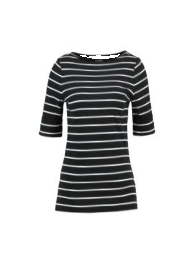
\includegraphics[width=2cm]{figures/c2dw/000008_1.png}&
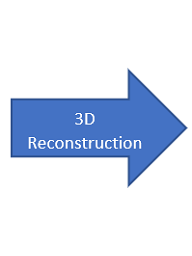
\includegraphics[width=2cm]{figures/arrow_recon.png}&
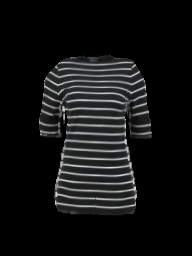
\includegraphics[width=2cm]{figures/c3drecon/000008_1_000303_0.png}&

\includegraphics[width=2cm]{figures/image/000303_0.jpg}&
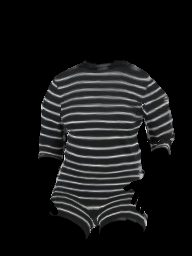
\includegraphics[width=2cm]{figures/c3dwfull/000008_1_000303_0.png}&
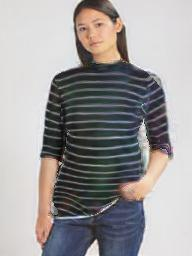
\includegraphics[width=2cm]{figures/try-on/000008_1_000303_0.jpg}\\


\includegraphics[width=2cm]{figures/c2dw/000005_1.png}&
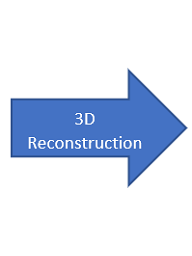
\includegraphics[width=2cm]{figures/arrow_recon.png}&
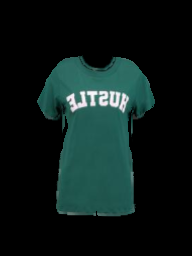
\includegraphics[width=2cm]{figures/c3drecon/000005_1_000303_0.png}&

\includegraphics[width=2cm]{figures/image/000303_0.jpg}&

\includegraphics[width=2cm]{figures/c3dwfull/000005_1_000303_0.png}&

\includegraphics[width=2cm]{figures/try-on/000005_1_000303_0.jpg}\\

  Cloth input(2D)&&Cloth(3D)&Target&Cloth(Warped)&Try-on\\

\end{tabular}

    \caption{We reconstruct a 3D cloth model from single 2D cloth image. Then, given a target human image, we transfer the reconstructed 3D cloth model properties to the target human image, and render the warped cloth as in 3D deformed. Finally, we blend the rendered cloth into the target human and generate virtual try-on output image.}
    \label{fig:summary}
\end{figure*}



\section{Introduction} \label{section:intro}


Online fashion market has been growing rapidly every year. Unlike electronics, which makes it easy to standardize functions and performances, fashion apparels have infinite variations in style, forms, colors, texture, and materials.  Also the difference between personal preferences is huge. As a result, clothing purchasing decisions are very difficult to make with current non-customized information, like the cloth and models' try fit images. Therefore, virtual try-on (VTON) is a highly demanding technology for the online shopping. 

The early VTON technologies were based on 3D computer graphics technology that uses 3D models for a target human and clothing, which are usually expensive and difficult to obtain. Therefore, recently 2D image-based VTON technologies are being studied in academia and industry, fueled by the recent advances in computer vision technologies based on deep learning (DL). 

There have been many assumptions in problem settings from the general conditional human image generation related to virtual try-on applications. We consider the one with a try-on cloth and target human image is a practical condition which is assumed in many papers VITON\cite{Han2017VITONAI}, CP-VTON\cite{Wang2018TowardCI} , and the following  \cite{Sun2019ImageBasedVT,Yu_2019_ICCV}. Therefore, we also consider the virtual try-on problem that uses the try-on clothes and human images and generates a new synthetic image that the target human replaced the current top or bottom cloth with the try-on cloth. In this paper, we limit our application to top cloth only due to the restricted data set. However, we consider that the bottom, e.g. pants cases would be easier than top cloth cases.


\begin{figure}[t]
\centering
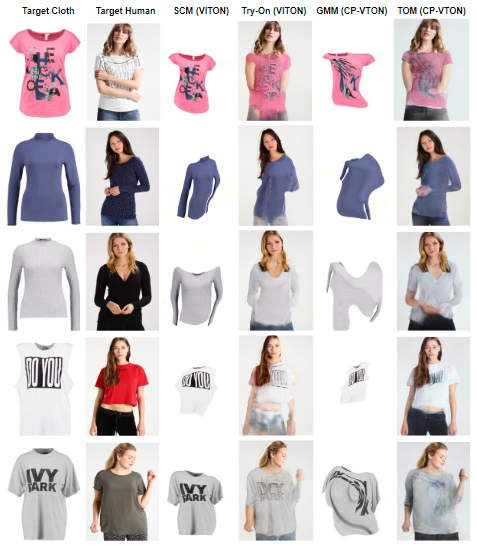
\includegraphics[scale=0.6]{figures/2dvton_diff.png}
\caption{Failures of image-based 2D cloth deformations for Virtual Try-On (Different clothes pairs)}
\label{fig:2dvtondiff}
\end{figure}


The existing 2D image-based algorithms seemingly generate high quality virtual try-on results. However, our classified analysis on the cloth styles, human poses, and shapes reveals significant problems, illustrated in Figure \ref{fig:2dvtondiff} and \ref{fig:classified2DVTONresult}. One reason of the seemingly high quality in the existing algorithms are mainly due to the low complexity of the dataset, i.e., most clothes are short-sleeved, and mono-colored, and the poses of humans are mild. Specifically, the results with the long-sleeved clothing arms and body posed show far low qualities than the presented results in the respective papers\cite{Han2017VITONAI,Wang2018TowardCI}. We identified 5 major issues in the state-of-the-art CP-VTON\cite{Wang2018TowardCI} pipeline, some of which are tackled in the following papers\cite{Sun2019ImageBasedVT,Yu_2019_ICCV}. Firstly, the target try-on area is dependent upon current cloth shape. Especially, the neck area pixels are labeled as background and some body areas are occluded by hairs or accessories, which affects in cloth warping and blending. Secondly, all unintended parts other than target clothing area, i.e., face, bottom-clothes and legs should be preserved in blending stage. However, other body parts except face and hairs are missing in CP-VTON\cite{Wang2018TowardCI} human representation inputs and generated at blending stage, which is all right for general synthesis application, but not desirable in virtual try-on application (Figure \ref{fig:2dvtondiff}, \ref{fig:classified2DVTONresult}). Thirdly, the texture is often not vivid, which is due to the composition. Examining the original loss function of Try-on Module (TOM) network, the term for the composition alpha mask are poorly formulated as in simple regularization loss.   

\begin{equation}
L = c_1 | I_0-I_{GT} |+  c_2 L_{VGG}+c_3 |1-M_0 |        
\end{equation} 

Fourthly, since no label in the area of warped cloth is the same color as background, white colored clothes are confused and improperly processed in the blending stage (Fig. \ref{fig:2dvtondiff} (c))
Finally, Geometric Matching Module (GMM) using Spatial Transformer Network\cite{JaderbergSZK15} with TPS (Thin Plate Spline)\cite{Bookstein1989PrincipalWT} deformation cannot handle strong 3D deformation due to the target pose, also  generates artifacts due to the person representation inputs. For example, hands-up and folded arms.  Note that many errors in the warping stage are often hidden in the blending stage, especially when the target clothes are single-colored, which can be expected in practical conditions (Figure \ref{fig:2dvtondiff}, \ref{fig:classified2DVTONresult}).

In this paper, we focus on the last but most difficult problems that cannot be solved in pure 2D image-based algorithm. The 3D cloth deformation is inherently difficult for 2D warping method, including non-rigid one, like TPS algorithm, we propose to first reconstruct 3D model of try-on cloth, then apply the pose and shape transfer for the target human, and finally blending with unchanged image contents like the face, bottom cloth, and background. Therefore, one of main the tasks now is to reconstruct 3D cloth model from 2D try-on cloth image. 3D clothed body model reconstruction have been studied in previous works \cite{natsume2019siclope,saito2019pifu}, however it still needs significant improvements for general condition. Our key idea in this step is that, once we can control the human pose and body shape to become similar to the try-on cloth's, the 3D reconstruction process can be made much easier, and the reconstruction quality would be much higher than general pose and shape condition. Figure \ref{fig:summary} shows a summarized glimpse of our total approach.

Therefore, in the Section \ref{section:3dclothrecon}, we describe the 3D cloth reconstruction algorithm. We divide the reconstruction step into 2D matching of cloth to the standard body silhouette and the 3D reconstruction of cloth. The later 3D reconstruction step is done through the SMPLify\cite{Bogo2016SMPLify} algorithm for the SMPL 3D body model\cite{Loper2015SMPLAS}.  In Section \ref{section:clothtransfer}, we describe the blending method, where the 3D cloth models are transferred to the target human images, through SMPL body parameters of shapes and poses. Then the transferred 3D reconstructed cloth is rendered and blended to the target human image. In this step, we reused the 2D virtual try-on blending algorithm with the modification for the condition.  The sampled results from dataset are presented in Section \ref{section:clothtransfer} and the paper is concluded in Section \ref{section:conclusion}. In addition to our main study, we added the classified quality evaluation of the previous 2D image based virtual try-on algorithms for the completeness of the paper.


